\documentclass[twoside=false,paper=A4,DIV=calc,BCOR=15mm,twocolumn,footsepline]{scrartcl}
%\usepackage{hyphsubst}
%\HyphSubstIfExists{ngerman-x-latest}{%
%\HyphSubstLet{ngerman}{ngerman-x-latest}}{}
\usepackage[ngerman]{babel}

\usepackage{natbib}
\usepackage{scrpage2}
\usepackage{hyperref}


\hypersetup{
%    bookmarks=true,         % show bookmarks bar?
    unicode=false,          % non-Latin characters in Acrobat’s bookmarks
    pdftoolbar=true,        % show Acrobat’s toolbar?
    pdfmenubar=true,        % show Acrobat’s menu?
    pdffitwindow=false,     % window fit to page when opened
    pdfstartview={FitH},    % fits the width of the page to the window
    pdftitle={Inklusion},    % title
    pdfauthor={Norbert Reschke},     % author
    pdfsubject={Hans-Sachs-Berufskolleg},   % subject of the document
    pdfcreator={Texmaker 3.2.2},
    pdfproducer={Texlive 2007},   % creator of the document
    pdfproducer={Texlive 2007}, % producer of the document
    pdfkeywords={Schule} {Berufliche-Bildung}, % list of keywords
    pdfnewwindow=true,      % links in new window
	breaklinks=true,
    colorlinks=true       % false: boxed links; true: colored links
%    linkcolor=red,          % color of internal links
%    citecolor=green,        % color of links to bibliography
%    filecolor=magenta,      % color of file links
%    urlcolor=cyan           % color of external links
}
%\renewcommand*{\pagebackref}[1]{[#1]}



\pagestyle{scrheadings}
\clearscrheadfoot
%\lofoot{Norbert Reschke} \rofoot{\pagemark}
\def\norefoot{%
\href{mailto:norbert.reschke@googlemail.com}{Norbert.Reschke\tiny{@googlemail.com}}\begin{tiny}- \today \end{tiny}
}
\lofoot{\norefoot}\rofoot{\pagemark}
\lefoot{\norefoot}\refoot{\pagemark}

% scrartcl, scrreprt
%\usepackage{bookman}
\usepackage{txfonts} % txfonts -- Times-like fonts in support of mathematics
%\usepackage{pxfonts} % pxfonts -- Palatino-like fonts in support of mathematics
\usepackage[T1]{fontenc}
\usepackage[utf8x]{inputenc}
%[pagebackref=true,]



\usepackage{color}
\usepackage{framed}
\usepackage{graphicx}
\usepackage{caption}
%\usepackage{pstricks}

%\usepackage{fancyhdr}
%\pagestyle{fancy}
%\fancyhead[L]{Inklusion} %Kopfzeile links
%\fancyhead[R]{Norbert Reschke} %Kopfzeile rechts
%\fancyfoot[C]{\thepage} %Seitennummer

\definecolor{shadecolor}{rgb}{.8,.8,.8}
%\definecolor{shadecolor}{rgb}{.91,.91,.85}
%\definecolor{shadecolor}{rgb}{1,.9,.6}

\newcommand{\Quelle}[1]{
\begin{small}
\begin{shaded}\noindent{#1}
\end{shaded}
\end{small}
}

%\setlength{\parindent}{0pt}
\setcounter{secnumdepth}{0}
%%%
\makeatletter
% Bilder skalieren
\def\ScaleIfNeeded{%
\ifdim\Gin@nat@width>\linewidth
\linewidth
\else
\Gin@nat@width
\fi
}
% Literatirverzeichnis
%\newcommand{\bibstyle@natdin}%
%       {\bibpunct{(}{)}{;}{a}{}{,~}
 %      \gdef\NAT@biblabelnum##1{\textbf{##1}\\}} %% \\ bewirkt Zeilenumbruch nach label-Ausgabe                                            
  % \bibstyle@natdin
%   \setlength{\bibhang}{4mm}
%\makeatother

\begin{document}
\section{Inklusion}
Inklusion bedeutet eine Schule für alle. Das ist eine griffige, aber zumindest unzureichende Kurzdefinition für ein pädagogisches Konzept in der weltweiten Bildung.
Boban/Hinz (2003) definieren Inklusion, als
\Quelle{... grundlegende Vorstellung eines Miteinanders der Verschiedenen; Ansatz einer Pädagogik der Vielfalt, die die Heterogenität der Menschen in all ihren Dimensionen wertschätzt und als Gewinn ansieht; hier verstanden als Erweiterung und Optimierung einer oft schwierigen Integrationspraxis; Leitbild einer \glqq Schule für alle\grqq ...}
\subsection{Ursprung und Umsetzung}
Der Bildungsbegriff kommt anscheinend aus dem anglo­amerika­nische Raum. In Changing Canadian Schools Perspectives on Disability and Inclusion beschreiben Porter/Richler (1991) ein Anfang der 90er schon etabliertes System in Kanada. Diane Richler beschreibt in Kapitel 2 Inclusive Education as Social Policy die Entwicklung in Kanada.
Die Wurzeln der Inklusion scheinen in den Konzepten zur Eingliederung von Menschen mit geistiger Behinderung zu liegen.
\Quelle{...Just as other minority groups in Canada have struggled for inclusion in the mainstream of society, so people who have a mental handicap, their families and their friends have engaged in a long campaign for inclusion. ...}

Richler verweist auf Bank-Mikelson und Nirje, die Ende der 60er in Skandinavien das principle of normalization für Menschen mit geistiger Behinderung entwickelt haben. In den 70ern wurde dieses Konzept von Wolfensberger in den USA und Kanada weiterentwickelt. Nirje und Wolfensberger sollen die Entwicklung der Inklusion in Kanada sehr beeinflusst haben.
\begin{center}
\begin{minipage}{\linewidth}
\centering
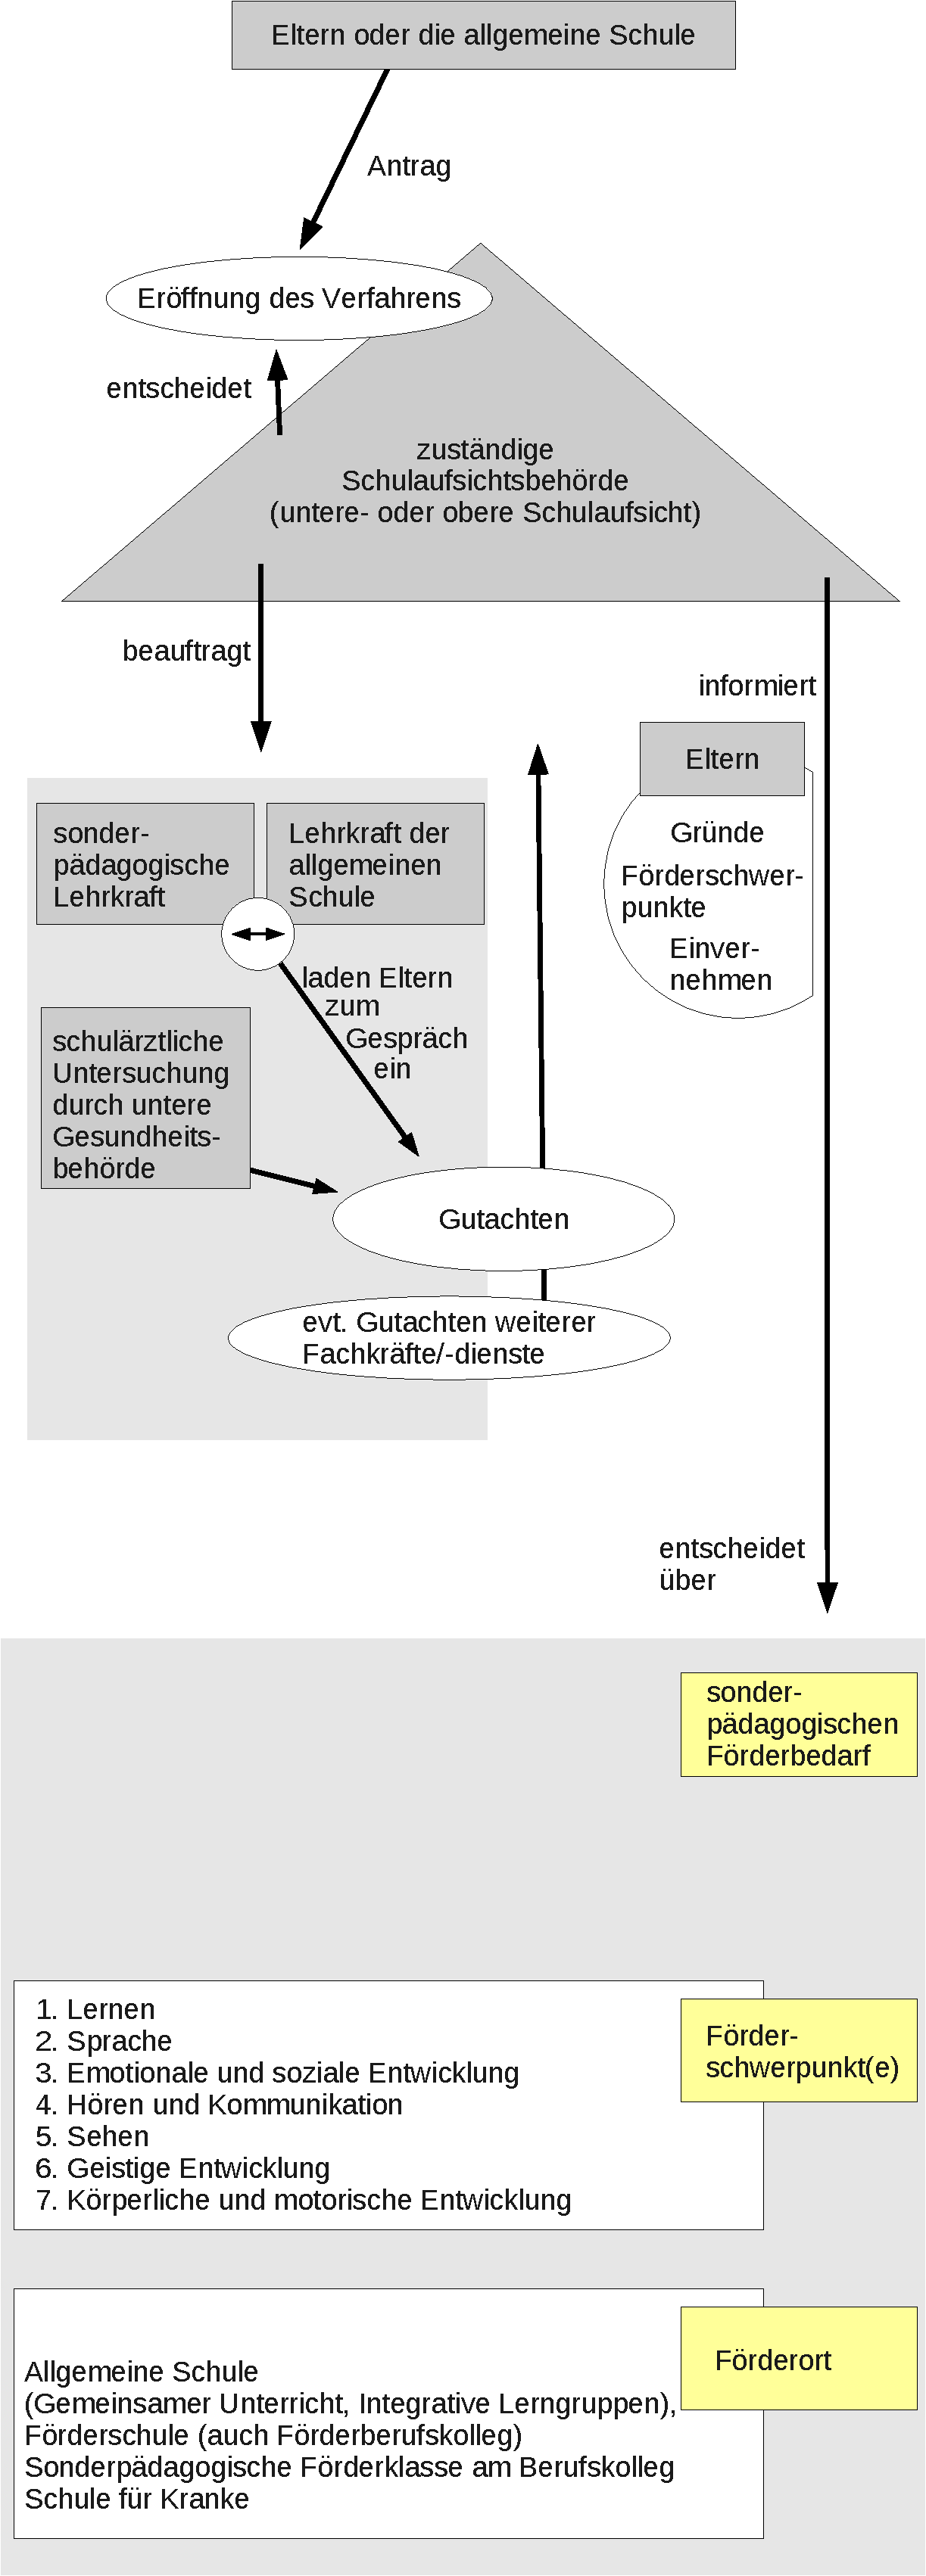
\includegraphics[scale=0.35]{AO-SF.pdf}
\captionof{figure}[]{AO-SF Verfahren}%
\end{minipage}
\end{center}
Richler führt auch die Widerstände gegen die Inklusion auf und den langen Zeitraum in dem sie entwickelt wurde
.\Quelle{...Therefore, the struggle in the 1940s,`50s and `60s undertaken by a small single-interest group to secure education for labelled children became the cause of a new, losely organized coalition. It now included people who had long been advocating for individuals with a mental handicap, and leaders from the human rights movement and from the field of education.
...\\
As bleak as the prospects were twenty years ago, the early 1990s have seen visitors from around the world look to Canada for models of inclusion.\\
... What happened in the years since 1970 to push integrated education onto the social policy agenda?
...
}
Unter anderem hat zum Erfolg der In­klusion in Kanada eine entsprechende Verfassungsänderung beigetragen.  
\Quelle{... In 1981, Canada repatriated its constitution and included in it a Charter of Rights and Freedoms. The original Charter prohibited discrimination on the basis of race, national or ethnic origin, colour, religion, sex or age. A 1985 amendment also prohibited discrimination on the basis of mental or physical disability.
...}

Diane Richler führt, aus den gesammelten Erkenntnissen in 1991, vor allem den Kom­pe­tenz­zuwachs im Bereich der Kommunikation, der Konzentration und des Verhaltens auf.
\Quelle{...
Perhaps the most important aspect of participation in an integrated setting is that learning takes place in an environment which provides its own rewards and measures of success. Parents and teachers from across Canada consistently report that students who move from segregated to integrated systems demonstrate improvements in communication skills, concentration skills and demeanour. ...}

Wie auch den Zitaten zu entnehmen ist, haben zu dieser Zeit Porter und Richler die Begriffe In­te­gration und Inklusion synonym gebraucht. Dies gilt sowohl für den Titel der Buchausgabe, als auch innerhalb der englischen Fassung, der zwei­spra­ch­igen Ausgabe.

Demnach ist es anscheinend richtig davon auszugehen, dass Porter und Richler der Begriff selbst nachrangig erschien. Unabhängig davon, betonen einige Quellen die synonyme Verwendung der Begriffe inclusion, integration und mainstreaming im englischen Sprachraum, andere ordnen (möglicherweise rückwirkend) erweiternde oder entwickelnde Bedeutungen, vor allem im amerikanischen Sprachraum, zu. So seien, in der Bildung, die 70er geprägt von mainsteaming, die 80er von integration und die 90ern von inclusive education. In Europa ent­wickelte sich ab 1994 ein Diskurs, der ähnlich verlief. Es gab zunächst die synonyme Ver­wen­dung von Integration und Inklusion, zur Zeit werden die Begriffe abgegrenzt.  
\subsection{Salamanca Konferenz}
Seit der Salamanca Konferenz, Salamanca statement (1994), der Unesco und des spani­schen Bildungsministeriums, wird der Begriff inclusive education bzw. inclusion in der euro­päischen Bildung verwendet. Im deutschen Sprach­raum wurde der Begriff in der Über­setzung der Erklärung 1996 zunächst mit Integration und erst 2010 (rückwirkend) mit Inklusion wiedergegeben.

\Quelle{... \\
3. Das Leitprinzip, ... , besagt, dass Schulen alle Kinder, unabhängig von ihren physischen, intellektuellen, sozialen, emotionalen, sprachlichen oder anderen Fähigkeiten aufnehmen sollen. Das soll behinderte und begabte Kinder einschließen, Straßen- ebenso wie arbeitende Kinder, Kinder von entlegenen oder nomadischen Völkern, von sprachlichen, kulturellen oder ethnischen Minoritäten sowie Kinder von anders benachteiligten Randgruppen oder -gebieten. ...\\
Im Zusammenhang mit diesem Aktionsrahmen bezieht sich der Begriff "besondere pädagogische Bedürfnisse" auf all jene Kinder und Jugendliche, deren Bedürfnisse von Behinderungen oder Lernschwierigkeiten herrühren. ... \\
Schulen müssen Wege finden, alle Kinder erfolgreich zu unterrichten, auch jene, die massive Benachteiligungen und Behinderungen haben. Es besteht wachsende Übereinstimmung darüber, dass Kinder und Jugendliche mit besonderen pädagogischen Bedürfnissen in jene Unterrichtsabläufe integriert werden sollen, die für den Großteil aller Kinder eingerichtet werden. Das hat zum Konzept inklusiver Schulen geführt. Die Heraus­forder­ung an inklusive Schulen ist es, eine kindzentrierte Pädagogik zu entwickeln, die in der Lage ist, alle Kinder, auch jene, die schwere Be­nach­tei­li­gungen und Behin­der­ungen haben, erfolgreich zu unterrichten. Der Wert solcher Schulen liegt nicht nur darin, dass sie alle Schüler und Schülerinnen mit qualitätsvoller Bildung versorgen können; ihre Einrichtung ist ein wesentlicher Schritt dahin, dass diskriminierende Haltungen verändert und Gemeinschaften geschaffen werden, die alle willkommen heißen, und dass eine inklusive Gesellschaft entwickelt wird. Eine Änderung der sozialen Perspektive ist zwingend notwendig. Viel zu lange wurden die Probleme von Menschen mit Behinderung durch eine behindernde Gesellschaft verursacht, die deren Schwächen mehr Beachtung geschenkt hat als den Stärken.
...}
\subsection{Behindertenrechtskonvention}
In der englischen (und spanischen Fassung) der Behindertenrechtskonvention - Convention on the Rights of Persons with Disabilities (2006) wird Inklusion eindeutig benannt:
\Quelle{...
Article 24 Education 
1. States Parties recognize the right of persons with disabilities to education. With a view to realizing this right without discrimination and on the basis of equal opportunity, States Parties shall ensure an inclusive education system at all levels and lifelong learning directed to: 
(a) The full development of human potential and sense of dignity and self-worth, and the strengthening of respect for human rights, fundamental freedoms and human diversity; 
(b) The development by persons with disabilities of their personality, talents and creativity, as well as their mental and physical abilities, to their fullest potential; 
(c) Enabling persons with disabilities to participate effectively in a free society. 

2. In realizing this right, States Parties shall ensure that: 
(a) Persons with disabilities are not excluded from the general education system on the basis of disability, and that children with disabilities are not excluded from free and compulsory primary education, or from secondary education, on the basis of disability; 
(b)  Persons with disabilities can access an inclusive, quality and free primary education and secondary education on an equal basis with others in the communities in which they live; 
(c) Reasonable accommodation of the individual’s requirements is provided; 
(d) Persons with disabilities receive the support required, within the general education system, to facilitate their effective education; 
(e) Effective individualized support measures are provided in environments that maximize academic and social development, consistent with the goal of full inclusion. 

3. States Parties shall enable persons with disabilities to learn life and social development skills to facilitate their full and equal participation in education and as members of the community. To this end, States Parties shall take appropriate measures, including: 
(a) Facilitating the learning of Braille, alternative script, augmentative and alternative modes, means and formats of communication and orientation and mobility skills, and facilitating peer support and mentoring; 
(b) Facilitating the learning of sign language and the promotion of the linguistic identity of the deaf community; 
(c) Ensuring that the eduStates Parties shall ensure an 
inclusive education system at all levels and lifelong learning directed to cation of persons, and in particular children, who are blind, deaf or deafblind, is delivered in the most appropriate languages and modes and means of communication for the individual, and in environments which maximize academic and social development. 

4. In order to help ensure the realization of this right, States Parties shall take appropriate measures to employ teachers, including teachers with disabilities, who are qualified in sign language and/or Braille, and to train professionals and staff who work at all levels of education. Such training shall incorporate disability awareness and the use of appropriate augmentative and alternative modes, means and formats of communication, educational techniques and materials to support persons with disabilities. 

5. States Parties shall ensure that persons with disabilities are able to access general tertiary education, vocational training, adult education and lifelong learning without discrimination and on an equal basis with others. To this end, States Parties shall ensure that reasonable accommodation is provided to persons with disabilities. }

Alle Unterzeichnerstaaten garantieren dieses Recht ihren Kindern, Jugendlichen und Erwachsenen. In der französischen Fassung (auch UN Amtssprache) und der deutschen Übersetzung taucht der Begriff Inklusion nicht auf. In der französichen Fassung wird insertion scolaire ver­wendet. inclusive education system wird in der deutschen Fassung der Konvention und im ent­sprechenden Gesetz über die Rechte von Menschen mit Behinderungen (2008) mit integratives Bildungssystem übersetzt.

In Kanada werden éducation intégratrice und inklusive education bis heute synonym ge­braucht, im französisch sprechenden Europa werden die Begriffe education intégratrice, education inclusive und insertion scolaire teilweise synonym, teilweise abgrenzend verwendet.

Artikel 24 s.o.
... States Parties shall ensure an inclusive education system at all levels and lifelong learning directed to:... 
... les États Parties font en sorte que le système éducatif pourvoie à l’insertion scolaire à tous les niveaux et offre, tout au long de la vie, des possibilités d’éducation qui visent: ...
... gewährleisten die Vertragsstaaten ein integratives Bildungssystem auf allen Ebenen und lebens­langes Lernen mit dem Ziel, ...
\subsection{Deutschland}
Der Begriff Inklusion oder Inklusive Bildung findet sich in keinem deutschen Bundesgesetz, der Begriff ist nicht im Schulgesetz NRW verankert, lediglich eine Verwaltungsvorschrift 
(VVzAO-SF) begründet im ABl. NRW. 01/11 S. 43 die Änderungen zum Gemeinsamen Un­terricht und Integrativen Lerngruppen (s. Abbildung 1, Seite 5) mit der Inklusion 
(Recherchestand 21.5.2011). 
Beschluss der KMK
Die Kultusministerkonferenz vom 18.11.2010 KMK (2010) stellt jedoch in ihrem Beschluss fest
...
Kinder und Jugendliche mit Behinderungen haben ein Recht auf schulische Bildung. Der Behindertenbegriff des Übereinkommens ist ein offener, an der Teilhabe orien­tierter Begriff. Er umfasst für den schulischen Bereich behinderte Schülerinnen und Schüler ohne sonder­päda­go­gischen Förderbedarf ebenso wie Schülerinnen und Schüler mit sonderpädagogischem Förderbedarf ...
...
Zentrales Anliegen der Behindertenrechtskonvention in der Bildung ist die Einbeziehung von Kindern und Jugend­lichen mit Behinderungen in das allgemeine Bildungs­system und damit auch das gemeinsame ziel­gleiche oder zieldifferente Lernen von Schülerinnen und Schülern mit und ohne Behinderungen (vgl. Art. 24 Abs.1 VN-BRK) in der allgemeinen Schule¹. Eine solche inklusive Bildung ist ein ständiger Prozess, der hochwertige Bildung für alle gewährleisten soll. Gruppen, in denen Vielfalt anerkannt und wertgeschätzt wird, bieten Chancen für alle Kinder, ihre Kompetenzen weiterzuentwickeln. Die Länder stellen sich ausdrücklich diesen Herausforderungen und dem damit verbundenen pädagogischen Perspektivwechsel 
bezogen auf Kinder mit Behinderungen. 

1 Allgemeine Schulen sind die allgemein bildenden und die berufsbildenden Schulen ohne Förderschulen oder Förderzentren. 
Zusammenfassung
Einige Quellen, insbesondere Wernstadt (2010), legen den Verdacht nahe, dass im Ringen um den Begriff und die Auslegung der Behinderten­rechtskonvention und die daraus resultierenden Konsequenzen, festgefahrene parteipolitische und/ oder bildungspolitische Interessen die in­haltliche Diskussion überlagern. Aus diesem Grund scheinen Einzelne, bis hin zu Verbänden, den Begriff in Ihrem Sinne besetzen zu wollen.
Inklusion soll umgesetzt oder verhindert werden, obwohl der Be­griff und die Inhalte, bei vielen Pädagogen und den betroffenen Schülern und Eltern nicht an­ge­kommen sind.

Zunächst sollten die Inhalte und das Konzept dargestellt werden, dies haben Boban/Hinz für den deutschen Sprachraum getan. Sie haben mit der Übersetzung und Adaption des index for inclusion Schlüsselkonzepte dargestellt, einen Rahmen für die Analyse zu strukturiert, Mater­ial­ien für die Analyse und den Index-Prozess auf­geführt.
Changing Canadian Schools Perspectives on Disability and Inclusion (Porter/Richler) ist für eine Akzeptanz des Begriffs, der Inhalte des Konzeptes und die Darstellung der Widerstände in der Um­setzung sehr nützlich. Eine deutsche Übersetzung existiert leider nicht, das Original ist nur noch als Kopie und ge­braucht im Um­lauf.

Zuletzt noch einmal der Versuch einer Definition im Kontext von Bildung:
Inklusion beschreibt das ratifizierte Recht auf Bildung für alle. Menschen werden inner­halb gleicher allgemeiner Schulformen in der­selben Lerngruppe unterrichtet. Dabei ist die Unterschiedlichkeit der Einzelnen, Grund­lage der Entwicklung der Kompetenzen aller.

Boban, Ines \& Hinz , Andreas (2003): Index für Inklusion Lernen und Teilhabe in der Schule der Vielfalt entwickeln: Martin-Luther-Universität Halle-Wittenberg 
(online verfügbar unter http://www.eenet.org.uk/resources/docs/Index%20German.pdf)

Convention on the Rights of Persons with Disabilities (2006): Convention on the Rights of Persons with Disabilities and Optional Protocol: UNITED NATIONS 
(online verfügbar unter http://www.un.org/disabilities/documents/convention/convoptprot-e.pdf)

Gesetz zu dem Übereinkommen der Vereinten Nationen vom 13. Dezember 2006 über die Rechte von Menschen mit Behinderungen sowie zu dem Fakultativprotokoll vom 13. Dezember 2006 zum Übereinkommen der Vereinten Nationen über die Rechte von Menschen mit Behinderungen (2008): Bundesgesetzblatt Jahrgang 2008 Teil II Nr. 35, ausgegeben zu Bonn am 31. Dezember 2008 
(online verfügbar unter http://www.un.org/Depts/german/uebereinkommen/ar61106-dbgbl.pdf)
KMK (2010) Pädagogische und rechtliche Aspekte der Umsetzung des Übereinkommens der Vereinten Nationen vom 13. Dezember 2006 über die Rechte von Menschen mit Behinderungen (Behindertenrechtskonvention - VN-BRK) in der schulischen Bildung
(online verfügbar unter\\
{\href{http://www.derwesten.de/staedte/muelheim/Abgebrannt-und-gesprengt-id3920655.html}{\nolinkurl{http://www.derwesten.de/staedte/muelheim/Abgebrannt-und-gesprengt-id3920655.html
}}}\\
\href{http://www.kmk.org/fileadmin/veroeffentlichungen_beschluesse/2010/2010_11_18-Behindertenrechtkonvention.pdf)}\\

Porter, Gordon L. \& Richler, Diane (Eds.) (1991): Changing Canadian Schools. Perspectives on Disability and Inclusion. North York, Ontario: Roeher Institute
(online verfügbar unter http://www.eric.ed.gov/ERICWebPortal/contentdelivery/servlet/ERICServlet?accno=ED341224)

% Salamanca-Statement (1994): The Salamanca Statement and Framework for Action on Special Needs Education. Adopted by the World Conference on Special Needs Education: Access and Quality, Salamanca, Spain, 7-10 June 1994. Paris (UNESCO)
% (online verfügbar unter http://www.unesco.de/fileadmin/medien/Dokumente/Bildung/Salamanca_Declaration.pdf)

% Wernstadt, Rolf (2010): Inklusive Bildung die UN-Konvention und ihre Folgen: Friedrich-Ebert-Stiftung, Berlin
(online verfügbar unter http://library.fes.de/pdf-files/studienfoerderung/07621.pdf)



weitere online Quellen zur Inklusion, die zur Recherche herangezogen wurden:

% http://www.unesco.de/fileadmin/medien/Dokumente/Bibliothek/InklusionLeitlinienBildungspolitik.pdf
% http://bidok.uibk.ac.at/library/unesco-salamanca.html
% http://www.un.org/Depts/german/uebereinkommen/ar61106-dbgbl.pdf

% http://en.wikipedia.org/wiki/Inclusion_%28education%29
% http://de.wikipedia.org/wiki/Inklusive_P%C3%A4dagogik

% http://www.bundestag.de/dokumente/textarchiv/2011/33790135_kw11_de_behinderung/index.html
% http://www.bundestag.de/dokumente/textarchiv/2011/33857489_kw12_pa_arbeitsoziales_pk/index.htm
% http://www.bundestag.de/bundestag/ausschuesse17/a13/kiko/Empfehlungen_und_Stellungnahmen/17-08_Stellungnahme_Kinder_mit_Behinderungen.pdf
% http://www.bundestag.de/bundestag/ausschuesse17/a11/aktuelles/handbuch_behindertenrechtskonvention.pdf

% http://www.schulministerium.nrw.de/BP/_Startseite/Aktuelles/Zwischenbericht_zum_Aktionsplan_NRW_Endfassung_nach_Billigung_Minister_Schneider_21_03_2011.pdf
% http://www.schulministerium.nrw.de/BP/Schulsystem/Statistik/2010_11/StatUebers373.pdfestag.de/dokumente/analysen/2009/behindertenrechtskonvention.pdf

% http://bidok.uibk.ac.at/library/sander-inklusion.html
% http://www.ance.lu/attachments/083_Sander%20Inklusionsp%C3%A4dagogik%2012-10-2006.pdf

% http://www.schulministerium.nrw.de/BP/Schulsystem/Statistik/2010_11/StatUebers373.pdf
% http://www.kmk.org/fileadmin/pdf/Statistik/Dok_190_SKL.pdf
\end{document}

